\section{Électromigration}
\begin{figure}[h]
    \begin{center}
        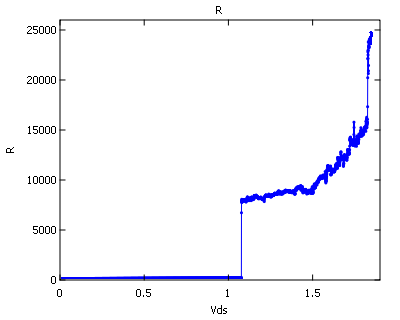
\includegraphics[width=150px]{Images/Image_Electromigration_1.png}
        \caption{La caractéristique R = f (V$_{ds}$)}
        \label{fig:}
    \end{center}
\end{figure}
On envoie un rampe de tension allant de 50mV à 2,5V avec une vitesse de 5mV/s.
L’énergie est dissipé par effet Joule et induit des vibrations du réseau cristallin. Après 1,2V  on commence à casser petit à petit la jonction jusqu’à créer le nanogap. Expérimentalement on observe Rmax=12,9kOhm pour un unique canal d’or et Rmax=25kOhm au moment de la formation du nanogap. On arrête donc l’électromigration lorsque l’on atteint R=25kOhm.
Grâce au système de mesure en temps réel on peut obtenir facilement la courbe R = f(Vds). Si l’électromigration est réussie on obtient une courbe du type de celle ci dessus, il est possible cependant que le nanofil soit déjà endommagé avant électromigration (résistance déjà de l’ordre de quelques kOhms). 

La mobilité des atomes est activée par la température. Localement (au niveau du nanogap) la température est de l’ordre de 400K lors de l’électromigration \cite{11}. Cependant l’arrêt de l’électromigration en une microseconde, et les dimensions concernées très faibles empêchent pas une élévation globale de l’échantillon en température.
\section{Observation du blocage de Coulomb}
Pour savoir si une molécule de C60 est tombé dans le nanogap, On trace la caractéristique I(V) pour différentes valeurs de la tension de grille Vg. L’influence de la boite quantique produira différentes caractéristiques, au contraire les caractéristiques seront toutes confondues si le gap est vide.
 Notons bien qu’il faut toujours utiliser des rampes de tensions entre la connexion et la déconnexion pour ne pas casser les fronts montants ou descendants en voyant des fronts d’une amplitude de 1V.
 \begin{figure}[h]
    \begin{center}
        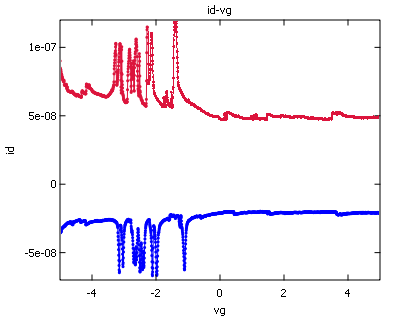
\includegraphics[width=150px]{Images/Image_Blocage_Coulomb_1.png}
        \caption{Id=f(Vg) on observe bien des pics de Coulomb (ici il pourrait s’agir d’un unique pic)}
        \label{fig:}
    \end{center}
\end{figure}
Sur la courbe Vds(Vg) on cherche à observer les diamants de Coulomb. Les différents pics mesurés doivent être également présents lorsqu’on envoie un tension drain-source négative, on est alors certain d’avoir non pas du bruit mais bien un pic lié au blocage de Coulomb.
Malheureusement nous n’avons pas pu obtenir des diamants de Coulomb exploitables. Selon Franck Balestro, un transistor sur 100 donne des résultats d’une bonne qualité.

\section{Quelques cas particuliers}
Après ces considérations générales étudions quelques cas particuliers, et plus précisément des observations obtenues lorsque des problèmes ont été rencontrés au cours de l’expérience.
\begin{table}[h!]
\begin{tabular}{c l}
    \begin{minipage}{0.25\textwidth}
      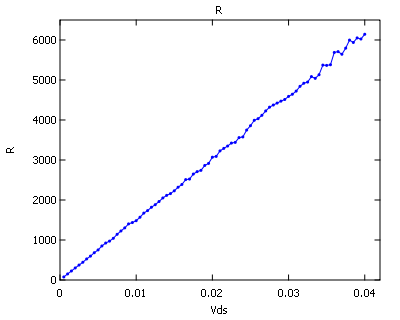
\includegraphics[width=\linewidth]{Images/Nanofil_Emdommage.png}
    \end{minipage} &
    \begin{minipage}{0.7\textwidth}
        \paragraph*{Nanofil endommagé avant électromigration\\}
    Dans ce cas, le nanofil a déjà été endommagé avec que l'on effectue l’électromigration. La résistance du fil est donc constante. Cependant, nous imposons une rampe de tension sur le nanofil avec le testeur sous pointe. On a d’après la loi d’Ohm R=U/I, donc si l’on impose une rampe de tension, on en aura une pour la résistance du nanofil. Ici, le transistor sera inutilisable.
    \end{minipage} \\

    \vspace*{0.5cm}\\
    \begin{minipage}{0.25\textwidth}
      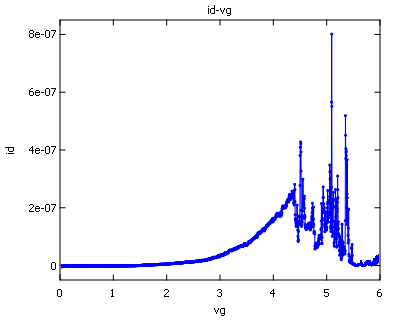
\includegraphics[width=\linewidth]{Images/Grille_Endommagee.png}
    \end{minipage} & 
    \begin{minipage}{0.75\textwidth}
        \paragraph*{Grille endommagée avant électromigration\\}
    On a toujours Id(Vg). On peut voir un fonctionnement de transistor, c’est à dire des pics de courants pour certaines valeurs de tension de grille mais on observe à partir d’une certaine valeur de Vg que le courant Id est toujours supérieur à 0. On a donc toujours un courant qui circule à travers la molécule. De plus, on observe beaucoup de bruit pour Vg supérieur à 4V. La grille est endommagée, le transistor ne fonctionnera pas normalement.
    \end{minipage} \\

    \vspace*{0.5cm}\\
    \begin{minipage}{0.25\textwidth}
      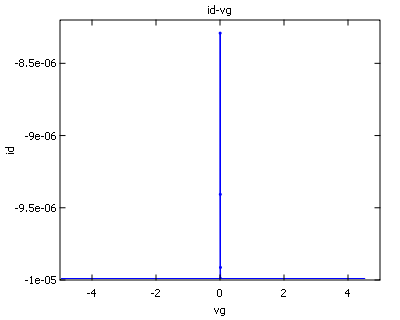
\includegraphics[width=\linewidth]{Images/Grille_Detruite.png}
    \end{minipage} & 
    \begin{minipage}{0.7\textwidth}
        \paragraph*{Grille détruite (au delà de Vg=7V on détruit la grille)\\}
    Quand on applique une trop grande tension à la grille, celle-ci claque. On n'a plus aucun contrôle sur le transistor à molécule unique. On a passage du courant quand Vg=0, sinon il n’y a pas de courant qui passe par le drain.
    \end{minipage}


\end{tabular}
\end{table}
